%%=============================================================================
%% Functionaliteiten
%%=============================================================================

\chapter{Functionaliteiten van het prototype}%
\label{ch:functionaliteiten}

Dit hoofdstuk beschrijft de belangrijkste functionaliteiten van het ontwikkelde prototype.
De focus ligt op eenvoud en ondersteuning van planning, gecombineerd met motivatie-elementen.


\section{Dagselectie en planning}

De applicatie laat toe om dagen te bekijken en een specifieke dag te selecteren om taken te plannen.
Deze aanpak ondersteunt studenten met ADHD doordat de focus op één dag tegelijk ligt, in plaats van een
overweldigend weekoverzicht.

\begin{figure}[h]
\centering
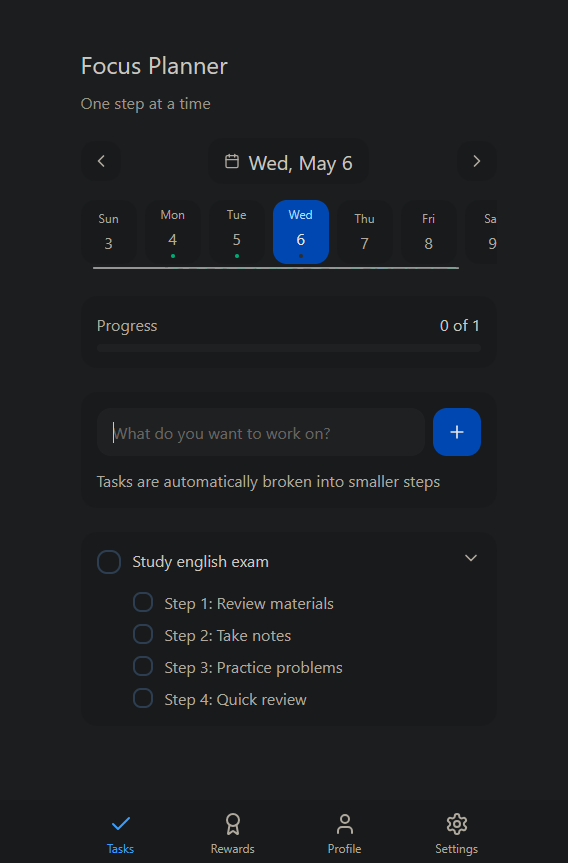
\includegraphics[width=0.55\linewidth]{tasks.png}
\caption[Dagoverzicht]{Voorbeeld van een dagoverzicht waarin geplande taken worden weergegeven.}
\label{fig:day-view}
\end{figure}


\section{Reward system: punten en streaks}

Wanneer een taak wordt voltooid, ontvangt de gebruiker punten. Daarnaast wordt een streak opgebouwd
wanneer de gebruiker meerdere dagen na elkaar actief taken voltooit. Dit biedt een directe beloning en
stimuleert consistent gedrag.

\begin{figure}[h]
\centering
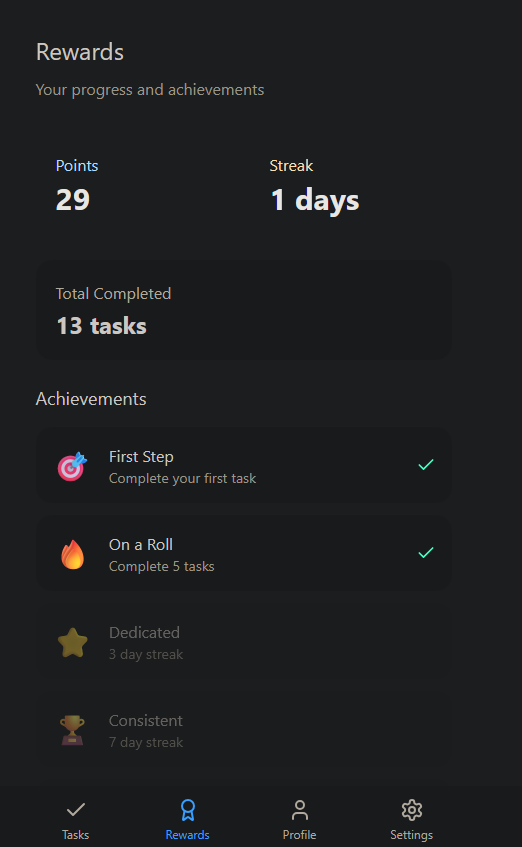
\includegraphics[width=0.55\linewidth]{streaks.png}
\caption[Streaks en punten]{Voorbeeld van de weergave van streaks en punten in het prototype.}
\label{fig:streaks}
\end{figure}


\section{Profielpagina}

Op de profielpagina kan de gebruiker een overzicht krijgen van behaalde punten, streaks en eventueel
andere statistieken. Dit ondersteunt het gevoel van vooruitgang.

\begin{figure}[h]
\centering
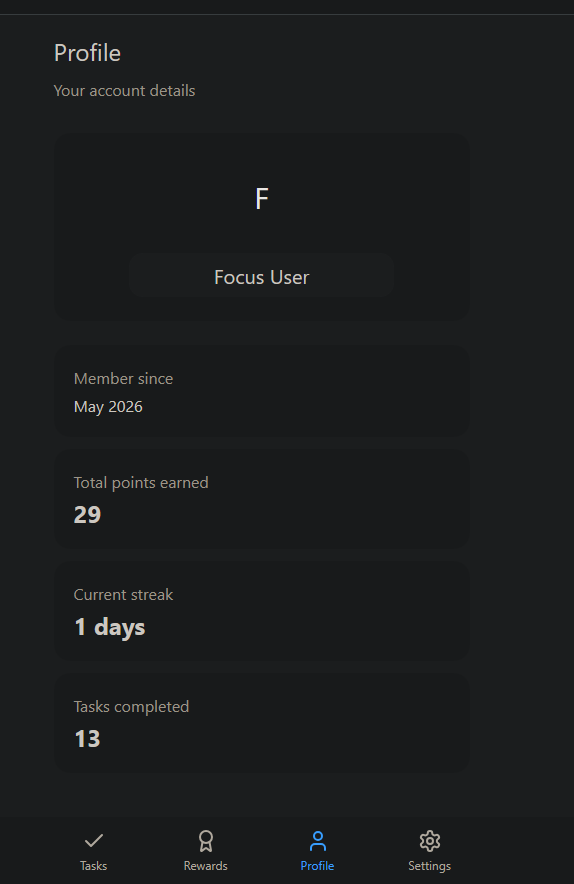
\includegraphics[width=0.55\linewidth]{profile.png}
\caption[Profielpagina]{Voorbeeld van de profielpagina met overzicht van voortgang.}
\label{fig:profile}
\end{figure}



\section{Instellingen}

De instellingenpagina biedt de mogelijkheid om persoonlijke voorkeuren te beheren. In dit prototype
blijven de instellingen beperkt om de eenvoud te bewaren.

\begin{figure}[h]
\centering
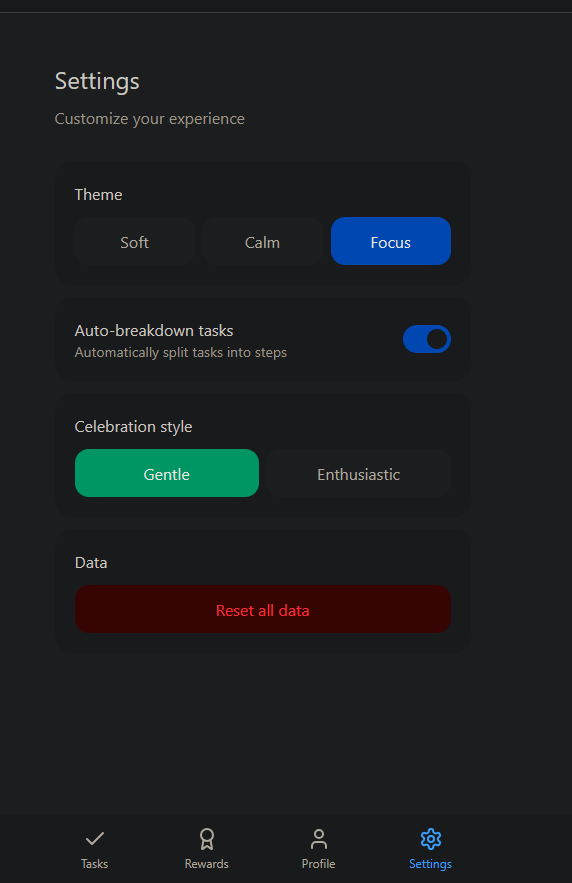
\includegraphics[width=0.55\linewidth]{settings.png}
\caption[Instellingen]{Voorbeeld van het instellingenmenu.}
\label{fig:settings}
\end{figure}

